TRITIUM-Aveiro is a proposal for the final TRITIUM detector module. This prototype, shown in Figure \ref{fig:TritiumAveiro0}, was designed and built in the University of Aveiro. It consists of a PTFE vessel, shown in Figure\ref{fig:TeflonStructureFibersTritiumAveiro0}, with an internal cylindrical hole of $43~\mm$ diameter and $18~\cm$ length.
\begin{figure}[h]
\centering
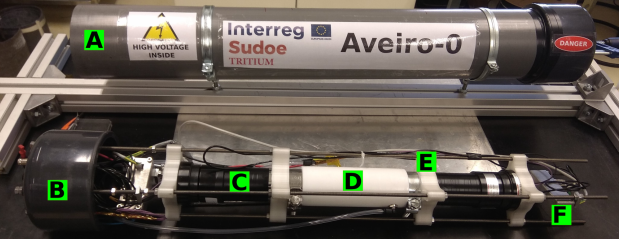
\includegraphics[scale=0.4]{5Prototypes/53FinalPrototypes/531TritiumAveiro/GeneralViewOfAveiroPrototype.png}
\caption{TRITIUM-Aveiro prototype. A and B are the PVC structure, C is the PMT, D is the PTFE vessel, E is the 3D printer piece and F is the electronics.\label{fig:TritiumAveiro0}}
\end{figure}
\begin{figure}[h]
\centering
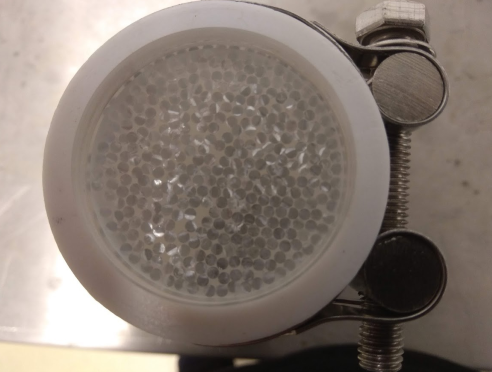
\includegraphics[scale=0.6]{5Prototypes/53FinalPrototypes/531TritiumAveiro/TeflonVessel_Fibers.png}
\caption{PTFE vessel and fiber bundle used in TRITIUM-Aveiro prototype.  \label{fig:TeflonStructureFibersTritiumAveiro0}}
\end{figure}
This vessel contains $360$ BCF-10 uncladded scintillating fibers of $180~\mm$ length from Saint-Gobain \cite{DataSheetBCF12Fiber}, which are similar to the BCF-12 fibers except the diameter and the attenuation length ($2.2~\meter$ for BCF-10 and $2.7~\meter$ for BCF-12). The scintillating fibers are stacked within the PTFE vessel in the maximum number that allows water to flow around them. These fibers were cleaved with the device described in section \ref{sec:CharacterizationScintillatingFibers}, but they were neither polished nor cleaned because the automatic polishing machine was not yet developed and it was not feasible to polish 360 fibers by hand. The PTFE vessel is totally closed and a water inlet and outlet were installed to allow a constant water flux through it. Two PMMA $10~\mm$ thick windows located at both ends of the fiber bundle are used to read out the fibers. Two clamps are used to make a tight junction of the PTFE walls and the PMMA windows. PMMA was chosen for its optical properties, especially its transmission coefficient which is larger than $95\%$ at the scintillating fiber wavelength. Two R2154-02 2" PMTs from Hamamatsu \cite{DataSheetPMTsAveiro}, shown in Figure \ref{fig:TritiumAveiro0}), are used to read out this prototype in coincidence. The PMT quantum efficiency is $26\%$ at $\lambda=430~\nano\meter$ and the HV was set at $-1500~\volt$. The PMTs are optically coupled to the PMMA windows through optical grease \cite{OpticalGrease}. The Aveiro prototype and its electronics were arranged in a structure composed of several clamps and four stainless-steel screws locked to an external PVC structure. This structure protects the prototype from physical damage and provides a light-tight operation environment. Only one prototype was built, which was designed to be installed in the Arrocampo dam. Two graphical interfaces were developed to control the PMT power supply and the data adquisition, respectively. 

Measurements to characterize the detector were carried out in the I3N and LARUEX laboratories. The prototype was in first place filled with pure water to measure the background and next with a radioactive liquid tritium solution of $30~\kilo\becquerel/\liter$ activity, which was used to measure the prototype efficiency and MDA. The volume of pure water and tritium solution used in TRITIUM-Aveiro prototype was $58~\milli\liter$. 

%The energy distribution of single photons of the PMT dark current was measured. To avoid environmental light detection, the TRITIUM-Aveiro prototype was removed and the measurement was carried out only with the PMTs, the windows of which were covered with black caps. The output signal of the PMTs were digitalized, shaped and pulse-height measured by a CAEN V1724 digitalizer \cite{CAENV1724}. The single-photon energy distribution of both PMTs fitted to a Gaussian function, is shown in Figure \ref{fig:SinglePhotonEnergyDistribution}. Due to the electrical noise of the PMT, the low energy tail was extrapolated (dashed line).

%\begin{figure}[h]
%\centering
%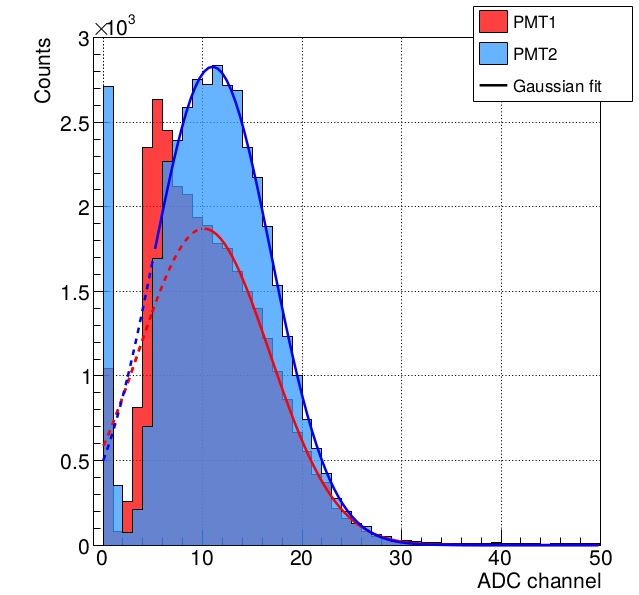
\includegraphics[scale=0.45]{5Prototypes/53FinalPrototypes/531TritiumAveiro/SinglePhotonEnergyDistribution.png}
%\caption{The single-photon energy distribution of both PMTs used in the TRITIUM-Aveiro prototype and their sum \cite{ExperimentalPaperCarlos}.\label{fig:SinglePhotonEnergyDistribution}}
%\end{figure}

%The distributions obtained deviates from Gaussian functions due to the noise in the low energy channels. As DRIM laboratory is not allowed to work with liquid radioactive source such as tritiated water, the first scintillating photons were produced by a $\ce{^{55}Fe}$ radioactive source since the energy of its $\gamma$ emission, $5.9~\keV$, is very close to the energy of tritium electrons. The TRITIUM-Aveiro prototype was coupled to both PMTs using optical grease and the radioactive source was placed inside the PTFE vessel. The prototype was not filled with water for this measurement. The spectra obtained are shown in Figure \ref{fig:55FeMeasurement}. A shift to higher energies is observed in the PMT2 data due to its higher gain and to the closer distance to the radioactive source.

%\begin{figure}[h]
%\centering
%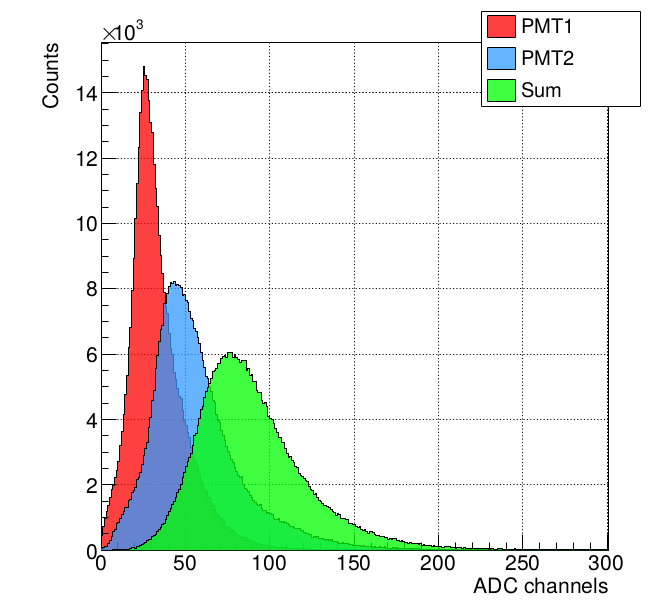
\includegraphics[scale=0.45]{5Prototypes/53FinalPrototypes/531TritiumAveiro/55FeMeasurement.png}
%\caption{Measurement of a $\ce{^{55}Fe}$ radioactive source with the TRITIUM-Aveiro prototype \cite{ExperimentalPaperCarlos}.\label{fig:55FeMeasurement}}
%\end{figure}


To quantify the background attenuation by a lead shield, measurements without shielding and with $2.5~\mm$ and $5~\mm$ lead shields were carried out at I3N. A background reduction by factors about 2 and 4 was obtained by the $2.5~\mm$ and $5~\mm$ lead shields, respectively, as shown in Figure \ref{fig:LeadShieldTest}.
\begin{figure}[h]
\centering
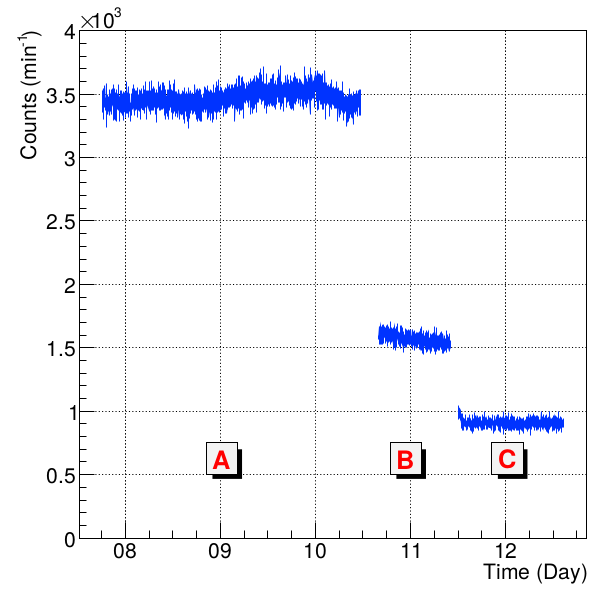
\includegraphics[scale=0.4]{5Prototypes/53FinalPrototypes/531TritiumAveiro/LeadShieldTest.png}
\caption{Background rate of the TRITIUM-Aveiro prototype. A) Without shielding. B) With a lead shield of $2.5~\mm$ thickness. C) With two lead shields of $2.5~\mm$ thickness each one \cite{ExperimentalPaperCarlos}.\label{fig:LeadShieldTest}}
\end{figure}

The prototype was installed in the LARUEX laboratory in order to be tested with tritiated water. The background was measured during 4 days with the prototype filled with pure water and shielded by $5~\cm$ lead. The events were grouped in $1$ minute time bins and the data were fitted to a Gaussian function as shown in Figure \ref{fig:BackgroundTritium1min}. An average rate of $540~\min^{-1}$ with a standard deviation of $\sigma_{Nb}=23~\min^{-1}$ was obtained. To calculate the MDA, the detection limit concepts developed by Lloyd A. Currie \cite{CurieLimit} were applied. The minimum number of net counts with a probability of a false-negative less than $5\%$ is given by,
\begin{equation}
N_D = 4.65 \cdot{}\sigma_{Nb} + 2.71 = 111~\min{}^{-1}
\label{eq:EquationNetCounts}
\end{equation}
which corresponds to a critical level of 
$$L_C = 2.33\cdot{}\sigma_{Nb}=53 ~\min{}^{-1}$$
$L_C$ and $N_D$ are calculateed after background subtraction. Therefore, the critical level $L_C'$ and the minimum count rate distinct from the background $N_D'$ are $$L_C'=540+53 = 593~\min{}^{-1}$$ and $$N_D'= 540+111=651~\min{}^{-1}$$
\begin{figure}
\centering
    \begin{subfigure}[b]{0.45\textwidth}
    \centering
    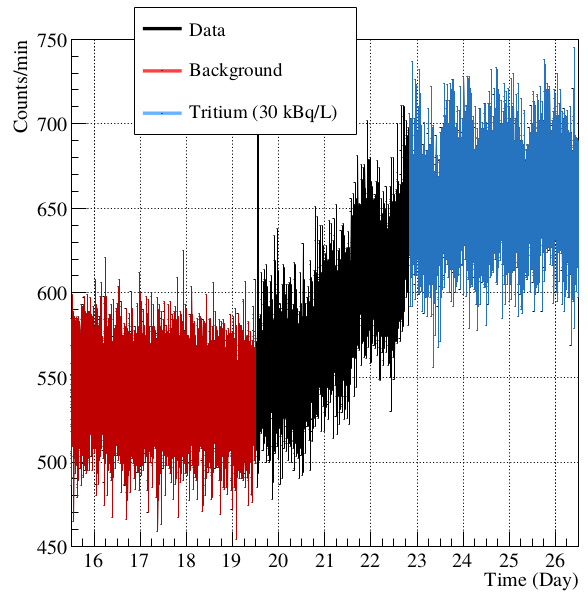
\includegraphics[width=\textwidth]{5Prototypes/53FinalPrototypes/531TritiumAveiro/Tritium_1min.png}  
    \caption{\label{subfig:MeasurementInRealTime}}
    \end{subfigure}
    \hfill
    \begin{subfigure}[b]{0.45\textwidth}
    \centering
    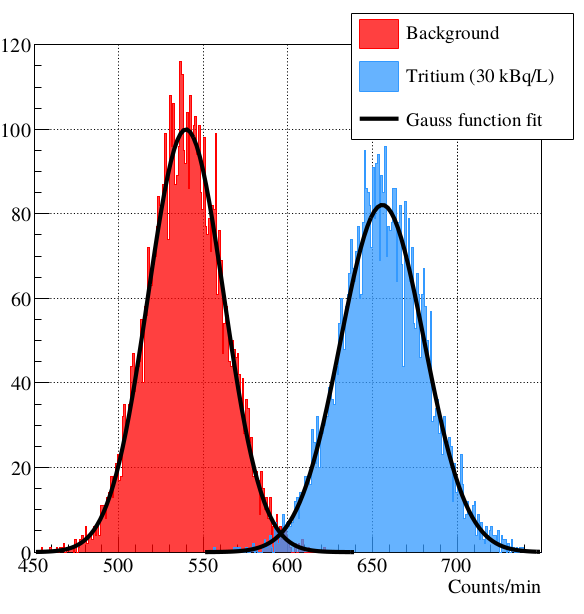
\includegraphics[width=\textwidth]{5Prototypes/53FinalPrototypes/531TritiumAveiro/Tritium_Gaus_1_min.png}  
    \caption{\label{subfig:DistributionofMeasurement}}
    \end{subfigure}
 \caption{Background and tritium liquid source ($29.8~\kilo\becquerel/\liter$) with the TRITIUM-Aveiro prototype \cite{ExperimentalPaperCarlos}. a) Counts per minut measured as a function of time. b) Distribution of the acquired data.}
 \label{fig:BackgroundTritium1min}
\end{figure}
To find the MDA, tritiated water was slowly added  so that the tritium water activity increased continuously till reaching the $N_D'$ value. A rate of $(656 \pm 26)~\min^{-1}$ was obtained that corresponds to a MDA=$(29.8\pm 3.6)~\kilo\becquerel/\liter$ measured with a Quantulus LSC.

The tritium detection efficiency was calculated from the ratio of the net tritium rate measured, $(1.9 \pm 0.6)~\sec^{-1}$, and the activity of the tritium source used, $29.8~\kilo\becquerel/\liter$. The tritium detection efficiency obtained is $$\eta=(6.5 \pm 1.9)\cdot{} 10^{-2}~\liter\:\kilo\becquerel^{-1}\second^{-1}$$ and the specific efficiency is
$$S=(1.6 \pm 0.5)\cdot{} 10^{-5}~\liter\:\kilo\becquerel^{-1}\second^{-1}\cm^{-2}$$ 
Comparing to the specific efficiency obtained with scintillating detectors in the literature (Table \ref{tab:PlasticScinTritium}), the specific efficiency of TRITIUM-Aveiro is close to the largest value $S<2.22~\liter\:\kilo\becquerel^{-1}\second^{-1}\cm^{-2}$ \cite{Hofstetter1, Hofstetter2}. TRITIUM-Aveiro has a lower specific efficiency than TRITIUM-IFIC-1, which could be attributed to the absent of polishing and cleaning of the fibers of this prototype. The efficiency uncertainty obtained is larger than for the first TRITIUM prototypes because of the shorter measurement time ($1$ minute instead of several hours). As the MDA depends directly on the background uncertainty, longer measurements are needed. The data for an integrated time of $60~\min$ is shown in Figure \ref{fig:Tritium60min}. The mean and the uncertainty of the measured background data are $3.186 \cdot{} 10^{4}~\hour^{-1}$ and $225~\hour^{-1}$ respectively. From the equation \ref{eq:EquationNetCounts}, values of $L_C=524~\hour^{-1}$ and $N_D=1048.96~\hour^{-1}$ are obtained. Assuming linearity between the activity and the counting rate, $N_D'=3.872\cdot{}10^4~\hour^{-1}$ corresponds to MDA=$(3.6 \pm 0.1)~\kilo\becquerel/\liter$. A daily oscillation is clearly observed in Figure \ref{fig:Tritium60min}, indicating that the measurements are affected by external light. This oscillation begins on the $19^{th}$ day when the water closed-circuit pump was installed, so it is likely that the light tightness of the system was affected.
\begin{figure}[h]
\centering
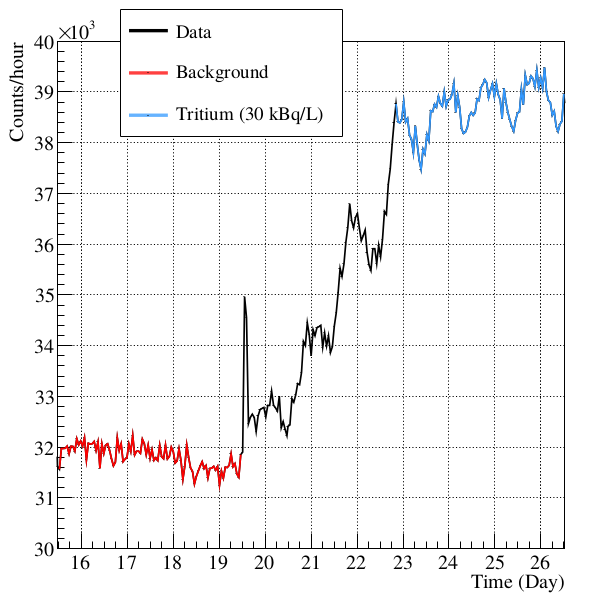
\includegraphics[scale=0.45]{5Prototypes/53FinalPrototypes/531TritiumAveiro/Tritium_60min.png}
\caption{Background and tritium liquid source counting rates measured with TRITIUM-Aveiro \cite{ExperimentalPaperCarlos} \label{fig:Tritium60min}.}
\end{figure}
This prototype was finally installed in the Arrocampo dam to test its functionality and to begin with the tritium level monitoring reported in section \ref{sec:ResultsArrocampo}.